% A workaround to allow relative paths in included subfiles
% that are to be compiled separately
% See https://tex.stackexchange.com/questions/153312/subfiles-inside-a-subfile-using-relative-paths
\providecommand{\main}{..}
\documentclass[\main/thesis.tex]{subfiles}
\externaldocument{previous}
\externaldocument{link}

\onlyinsubfile{\externaldocument{\main/tex/introduction}}

\begin{document}
\chapter{Local Community Detection}
\section{Local Community Detection Algorithm for Uncertain Networks}
\subsection{Local Modularity $\mathcal{UR}$ in Uncertain Networks}
Inspired by the local modularity $\mathcal{R}$ in deterministic networks, in order to solve the problem of detecting local communities with edge uncertainty, one intuitive approach is to convert the uncertain community detection problem into the deterministic scenario by using edge probability. In the uncertain scenario, the local modularity $\mathcal{UR}$ for uncertain networks can be defined as follows:
\begin{equation}
\mathcal{UR} = \frac{\mathbb{E}(\mathcal{B}_{in\_edge})}{\mathbb{E}(\mathcal{B}_{in\_edge})+\mathbb{E}(\mathcal{B}_{out\_edge})}
\label{UR-Local}
\end{equation}
where $\mathbb{E}(\mathcal{B}_{in\_edge})$ is the expected number of edges that connect boundary nodes and other nodes in $\mathcal{D}$, which can be represented as:
\begin{equation}
\mathbb{E}(\mathcal{B}_{in\_edge}) = \frac{1}{2}\sum_{\mathcal{V}_i\in \mathcal{B},\mathcal{V}_j\in \mathcal{B},i\neq j}\mathcal{P}_{i,j}+\sum_{\mathcal{V}_i\in \mathcal{B},\mathcal{V}_j\in \mathcal{C}}\mathcal{P}_{i,j}
\end{equation}
while $\mathbb{E}(\mathcal{B}_{out\_edge})$ is the expected number of edges that connect boundary nodes and nodes in $\mathcal{S}$, which can be represented as:
\begin{equation}
\mathbb{E}(\mathcal{B}_{out\_edge}) = \sum_{\mathcal{V}_i\in \mathcal{B},\mathcal{V}_j\in \mathcal{S}}\mathcal{P}_{i,j}
\end{equation}

After using $\mathcal{UR}$ to take the place of $\mathcal{R}$, we can use the algorithm mentioned in \cite{clauset2005finding,chen2009detecting} to find the local community for the input node. 
\subsection{Reviews of the Previous Method}
However, simply using $\mathcal{UR}$ to take the place of $\mathcal{R}$ and applying Clauset and Chen's original local community detection algorithm (as mentioned in Section \ref{Local-Community-Detection-Algorithms-Review}) will cause some problems. In uncertain networks, there are some noise edges between nodes, which may be generated by missed observations, misreporting or wrong inference. Although some of them are assigned low probability, they do not actually exist and can be regarded as noises. Due to these kinds of noises, if the algorithm starts from a node $\mathcal{V}_i$ in community $A$, the expansion step might fall into a different neighbor community $B$. Figure \ref{problem_example} shows an example.

\begin{figure}
\centering
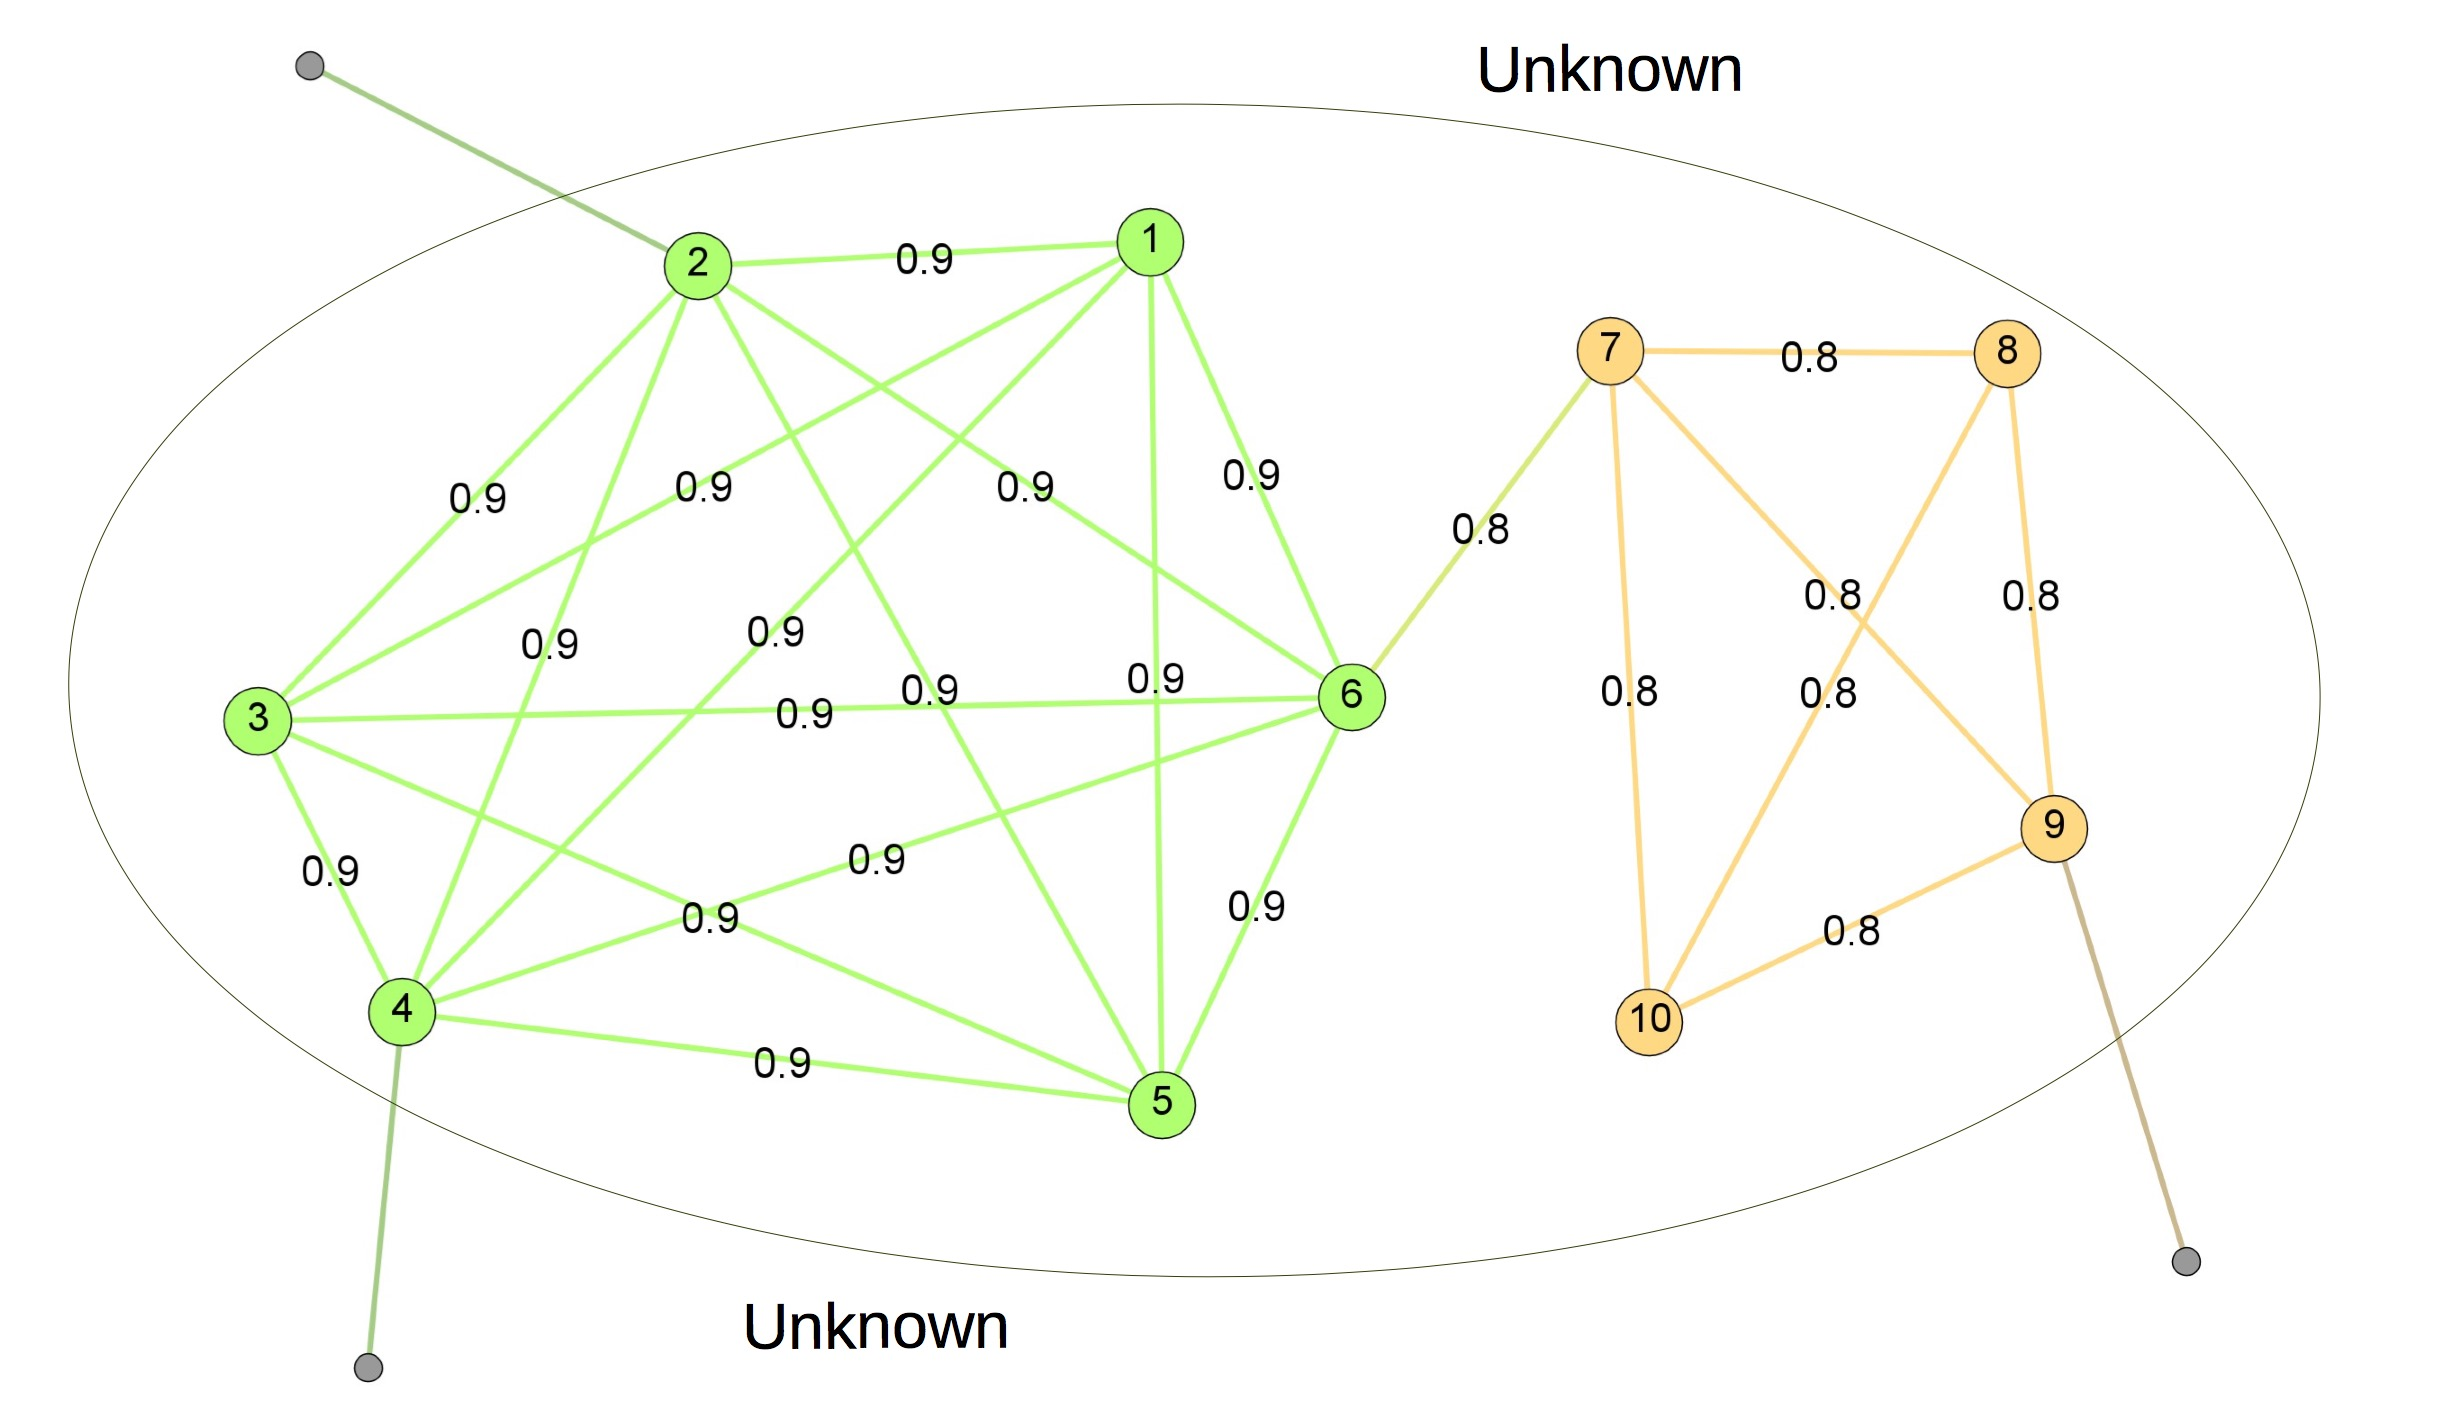
\includegraphics[scale = 0.12]{\main/img/toy_example.jpeg}
\caption{An example showing the problem when only using $\mathcal{UR}$ to find the local community.}
\label{problem_example}
\end{figure}

Community A is a 6-vertex clique, and the probability over edges in community A are all 0.9. Community B is a 4-vertex clique, and the probability over edges in community B are all 0.8. Besides these edges, there is an edge between node $\mathcal{V}_6$ and node $\mathcal{V}_7$ with a probability of 0.8. There are also some other edges between other nodes of community A and B and the unknown part of the network. If the start node is $\mathcal{V}_6$, we want to find the local community for node $\mathcal{V}_6$. The algorithm mentioned in \cite{clauset2005finding,chen2009detecting} starts the expansion step from the start node's neighbors and adds the node which results in the largest increase in $\mathcal{R}$ to the community. In this uncertain example, we use $\mathcal{UR}$ to take the place of $\mathcal{R}$. $\mathcal{V}_1$ to $\mathcal{V}_5$ and node $\mathcal{V}_7$ are all neighbors of $\mathcal{V}_6$, so they are all candidates. The $\mathcal{UR}$ of the community, after adding $\mathcal{V}_1, \mathcal{V}_3$ or $\mathcal{V}_5$, are all 
\begin{equation}
\frac{0.9}{4\times0.9+(4\times0.9+0.8)+0.9}=0.1011
\label{value-after-add-135}
\end{equation}
After adding node $\mathcal{V}_2$ or $\mathcal{V}_4$, the $\mathcal{UR}$ will be less than 0.1011 due to extra outward edges. The $\mathcal{UR}$ of the community after adding node $\mathcal{V}_7$ is 
\begin{equation}
\frac{0.8}{5\times0.9+3\times0.8+0.8}=0.1039
\end{equation}

The algorithm will add node $\mathcal{V}_7$ to $\mathcal{C}$ because it results in the largest increase in $\mathcal{UR}$. Then nodes $\mathcal{V}_8, \mathcal{V}_9, \mathcal{V}_{10}$ (or $\mathcal{V}_{10}, \mathcal{V}_9, \mathcal{V}_{8}$, because nodes $\mathcal{V}_8$ and $\mathcal{V}_{10}$ are exactly the same) will be added to $\mathcal{C}$ one by one. In this example, when we input the node $\mathcal{V}_6$, the algorithm will regard nodes $\mathcal{V}_6$ to $\mathcal{V}_{10}$ as node $\mathcal{V}_6$'s local community, while it should be nodes $\mathcal{V}_1$ to $\mathcal{V}_6$.

In this example, the structure of the network is clear, but the algorithm still makes a wrong decision. Chen also reported a similar problem in the deterministic network in \cite{chen2009local}, but he regarded these start nodes as periphery nodes and didn't provide local communities for these nodes. In other uncertain networks, there are more (noise) edges between communities, and the probability over some edges are low while others are high, which make the situation even more complex. In complex uncertain networks, more nodes will encounter the aforementioned problem and be grouped into their neighbor communities. We can not just simply regard these nodes as periphery nodes and report no community for them.
\subsection{Introduction of the New Measure $\mathcal{K}$}
The reason why the original algorithm does not perform well in uncertain networks is that $\mathcal{UR}$ only measures the sharpness of the boundary. However, in the uncertain scenario, the boundary between communities becomes less clear due to the appearance of noise edges. One main drawback of the local modularity $\mathcal{UR}$ is that it only cares about the nodes in $\mathcal{D}$ and pays no attention to the difference between shell nodes and unknown area's nodes. At this moment, though shell nodes are not part of the community, they can be regarded as the neighbors of the community, and they can give us extra information about the community. In the research of link prediction, people propose the measure called Common Neighbor (CN) to find the potential links. Researchers find that two nodes are more likely to form a link if they have many common neighbors. This idea can also be used in the local community detection problem. It's easy to understand that nodes in the same community share some common neighbors, even though they don't have direct links with each other. Inspired by this idea, in order to solve the existing problem in uncertain scenarios mentioned previously, a new measure $\mathcal{K}$ is introduced, which not only pays attention to nodes in $\mathcal{B}$, but also nodes in $\mathcal{S}$.
% while neglecting the nodes in $\mathcal{S}$.(Problems, maximize the links towards node in D and minimize links towards other part of graph, and pay no attention to the difference between shell nodes and unknown place's nodes. It's enough in deterministic scenario only care about nodes in D, but the boundary become less clear, so we may need extra information in S ) 
%At this moment, though shell nodes are not part of the community, they can be regarded as the neighbors(friends) of the community, and they can give us extra information about the community. It's easy to understand that people(nodes) in the same community share some common friends(neighbors), even though they don't know each other(direct link with each other). Inspired by this idea, in order to solve the existing problems in uncertain scenario mention aforementioned, a new measure $\mathcal{K}$ is introduced, which not only pay attention to nodes in $\mathcal{B}$, but also nodes in $\mathcal{S}$.
\begin{equation}
%\mathcal{K} = \mathbb{E}(N_{community\_node}) + \mathbb{E}(N_{shell\_node})
\mathcal{K}_i = \mathbb{E}(N_{i,in\_edge}) + \mathbb{E}(N_{i,shell\_edge})
\end{equation}
where $\mathbb{E}(N_{i,in\_edge})$ is the expected number of edges that connect candidate node $\mathcal{V}_i$ and other nodes in $\mathcal{D}$, which can be represented as:
\begin{equation}
\mathbb{E}(N_{i,in\_edge}) = \sum_{\mathcal{V}_j\in \mathcal{D}}\mathcal{P}_{i,j}
\end{equation}
while $\mathbb{E}(N_{i,shell\_edge})$ is the expected number of edges that connect candidate node $\mathcal{V}_i$ and other nodes in $\mathcal{S}$, which can be represented as:
\begin{equation}
\mathbb{E}(N_{i,shell\_edge}) = \sum_{\mathcal{V}_j\in \mathcal{S}}\mathcal{P}_{i,j}\cdot \mathcal{P}_{j,shell}
\end{equation}

\begin{equation}
\mathcal{P}_{j,shell} = 1-\prod_{\mathcal{V}_m\in \mathcal{D}}(1-\mathcal{P}_{j,m})
\label{update-probability}
\end{equation}
(Common Neighbor metric aims to measure how likely it is that two nodes are linked, and the new measure $\mathcal{K}$ aims to measure how likely it is that the candidate and the sub-community are in the same community.)
The new measure $\mathcal{K}$ aims to measure how close the relationship is between the candidate node and the existing community. The larger the value $\mathcal{K}$ is, the closer the relationship between the community and the candidate node will be. This measure will be used to choose which neighboring node should be added to $\mathcal{C}$ (and to $\mathcal{B}$, if necessary) in the first few steps. 
It is worth noting that:
\begin{enumerate}
\item $\mathbb{E}(N_{i,shell\_edge})$ is not simply the sum of probability over edges between candidate node $\mathcal{V}_i$ and nodes in $\mathcal{D}$, but it also cares about the true probability of at least one edge between shell node $\mathcal{V}_j$ and the existing community being present, which is denoted by $\mathcal{P}_{j,shell}$.
%\item In the definition of $\mathcal{K}$, we only care about edges between candidate node $\mathcal{V}_i$ and nodes in $\mathcal{D}$ and $\mathcal{S}$, but pay no attention to edges between candidate node $\mathcal{V}_i$ and other unknown parts of the graph. The node which is added to $\mathcal{C}$ should have as few edges towards the unknown part of the graph as possible. The reason why we don't introduce this term in the definition of $\mathcal{K}$ is because this part has already been reflected in the definition of $\mathcal{UR}$, which can be regarded as a part of $\mathbb{E}(\mathcal{B}_{out\_edge})$, and we don't use this term repeatedly. When two candidate nodes have the same $\mathcal{K}$, we will choose the node which can result in the largest increase in $\mathcal{UR}$. %We also tested 
%\item In the definition of $\mathcal{K}$, we didn't introduce ... Though the less, the better, it has already reflected in the definition of R, so we don't use it repeatedly. (and we have tested that introduce it will ruohua xingneng) example, the same, but we will choose from ... rather than ... because of R value
\item The start node is more likely to merge other communities' nodes at the first few steps of the discovery phase. With the increase in the number of nodes, the possibility of wrongly adding other communities' nodes will be significantly reduced, so $\mathcal{K}$ will only be mainly considered in the first few steps of the discovery phase ($\mathcal{K}$ will also be considered when $\mathcal{UR}$ ties in future steps). %(See Algorithm 1)
%\item The number 3 needs be checked. It is a tunable hyper-parameter. All experiments (except the one we researched on the choice of k) described later use 3.
%of a start node begins finding its local community
\end{enumerate}

In the example mentioned in Figure \ref{problem_example}, the $\mathcal{K}$ value for nodes $\mathcal{V}_1, \mathcal{V}_2, \mathcal{V}_3, \mathcal{V}_4, \mathcal{V}_5$ and $\mathcal{V}_6$ are calculated as follows:

\begin{equation}
\mathcal{K}_{i=1,2,3,4,5}=0.9+0.9\times0.9\times4=4.14
\end{equation}
\begin{equation}
\mathcal{K}_{i=7}=0.8
\end{equation}

$\mathcal{K}_{i=7}$ is smaller than $\mathcal{K}_{i=1,2,3,4,5}$, so we will first exclude node $\mathcal{V}_7$. As mentioned in Equation \ref{value-after-add-135}, the $\mathcal{UR}$ of the community after adding $\mathcal{V}_1, \mathcal{V}_3$ or $\mathcal{V}_5$ is 0.1011 while the $\mathcal{UR}$ of the community after adding $\mathcal{V}_2$ or $\mathcal{V}_4$ is less than 0.1011. The node added to the community $\mathcal{C}$ will be randomly chosen from nodes $\mathcal{V}_1, \mathcal{V}_3$ and $\mathcal{V}_5$.


\subsection{Full Algorithm Description} \label{Full-Algorithm-Description-local}
Similar to Clauset and Chen's greedy algorithm mentioned in Section \ref{Local-Community-Detection-Algorithms-Review}, our algorithm also firstly place the start node in the community. At each step, we sort candidate nodes based on their $\mathcal{K}$ (first few steps) or $\mathcal{UR}$ values (other steps). After all candidate nodes are sorted, the algorithm will add the first node (which can increase the community's $\mathcal{UR}$) to the community $\mathcal{C}$. This process will stop when there are no remaining nodes in $\mathcal{S}$ which can increase the community's $\mathcal{UR}$. It is worth noting that candidate nodes are sorted based on $\mathcal{K}$ value in the first few steps. However, the number of steps is not yet decided. It is a tunable hyper-parameter, and we use $\lambda$ to represent it. We will demonstrate how to find the optimal $\lambda$ in Section \ref{Hyper-Parameter-Evaluation-Local}. The full algorithm description can be found in Algorithm \ref{Local-Community-Identification-with-Edge-Uncertainty}.
% The full algorithm includes the \textbf{Discovery Phase} and the \textbf{Examination Phase}. In the discovery phase, one can sort candidate nodes based on their $\mathcal{K}$ (first a few steps) or $\mathcal{UR}$ values at other steps. After all candidate nodes are sorted, the algorithm will add the first node which can increase the community's $\mathcal{UR}$ to the community $\mathcal{C}$. This process will stop when there are no remaining nodes in $\mathcal{S}$ which can increase the community's $\mathcal{UR}$. In the examination phase, nodes in $\mathcal{C}$ which have more neighbors outside $\mathcal{C}$ than inside will be removed except the start node. Here, $\mathcal{V}_i^{in}$ denotes the expected number of edges between node $\mathcal{V}_i$ and other nodes within the community, while $\mathcal{V}_i^{out}$ denotes the expected number of edges between node $\mathcal{V}_i$ and nodes which do not belong to the community. Besides, it is worth noting that candidate nodes are sorted based on $\mathcal{K}$ value in the first a few steps in the discovery phase. However, the number of steps is not yet decided. It is a tunable hyper-parameter, and we use $\lambda$ to represent it. (We will demonstrate how to find the optimal $\lambda$ in Section 3.3.) The full algorithm description can be found in Algorithm 1.
%using $\mathcal{K}$ at first 3 steps and $\mathcal{UR}$ at future steps to evaluate the relationship between candidate node and the existing community,

%The full algorithm description is as follows:

\begin{algorithm}
  \KwData{A network $\mathcal{G}$, a start node $\mathcal{V}_0$ and number of steps $\lambda$.}
  \KwResult{A local community for $\mathcal{V}_0$}% and its quality score R.
  Add $\mathcal{V}_0$ to $\mathcal{D}$ and $\mathcal{B}$, add all $\mathcal{V}_0$'s neighbors to $S$, $\mathcal{UR} \leftarrow 0$\;
  %// \textbf{Discovery Phase}\;
  \Repeat{no new node is added to $\mathcal{D}$}{
  	Array $nodelist \leftarrow [ ]$\;
	\For{each $\mathcal{V}_i \in S$}{
        Compute $\mathcal{UR}_i$\; 
        // $\mathcal{UR}_i$ represents the $\mathcal{UR}$ value after adding node $\mathcal{V}_i$\;
        Compute $\mathcal{K}_i$\;
        Add $\mathcal{V}_i$ to $nodelist$\;
%         \If{$\mathcal{V}_i.K>threshold$}{
%         	Add $\mathcal{V}_i$ to $nodelist$\;
%         }
    }
        %Sort the node $\mathcal{V}_i \in S$ first by $K_i$, second by $R_i$\;
        \uIf{$|\mathcal{D}|<\lambda$}{
        Sort $nodelist$ first by $\mathcal{K}_i$, then by $\mathcal{UR}_i$\;}
        \Else{
        Sort $nodelist$ first by $\mathcal{UR}_i$, then by $\mathcal{K}_i$\;}
        // If some nodes have same $\mathcal{K}_i$ and $\mathcal{UR}_i$, break ties randomly\;
    \For{each $\mathcal{V}_i \in nodelist$}{
    	\If{$\mathcal{UR}_i>\mathcal{UR}$}{
        	$\mathcal{UR} \leftarrow \mathcal{UR}_i$\;
        	Add $\mathcal{V}_i$ to $\mathcal{D}$\;
            Remove $\mathcal{V}_i$ from $\mathcal{S}$\;
            Update $\mathcal{B}$, $\mathcal{D}$\;
            Update shell nodes possibility based on Equation \ref{update-probability}\;
            \textbf{break} for loop
        }
    }
  }
%   // \textbf{Examination Phase}\;
%   Array $community \leftarrow [n_0]$\;
%   \For{each $\mathcal{V}_i \in \mathcal{D}$}{
%     	\If{$\mathcal{V}_i \neq n_0$ \textbf{and} $\mathcal{V}_i^{in}>N_i^{out}$}{
%         	Add $\mathcal{V}_i$ to $community$\;
%         }
%     }
   \Return{$\mathcal{D}$}
  \caption{Local Community Identification with Edge Uncertainty}
  \label{Local-Community-Identification-with-Edge-Uncertainty}
   \end{algorithm}

% \begin{algorithm}
%   \KwData{A network $G$, a start node $\mathcal{V}_0$ and number of steps $\lambda$.}
%   \KwResult{A local community for $\mathcal{V}_0$}% and its quality score R.
%   Add $\mathcal{V}_0$ to $\mathcal{D}$ and $\mathcal{B}$, add all $\mathcal{V}_0$'s neighbors to $S$, $\mathcal{UR} \leftarrow 0$\;
%   // \textbf{Discovery Phase}\;
%   \Repeat{no new node is added to $\mathcal{D}$}{
%   	Array $nodelist \leftarrow [ ]$\;
% 	\For{each $\mathcal{V}_i \in S$}{
%         Compute $\mathcal{UR}_i$\; 
%         // $\mathcal{UR}_i$ represents the $\mathcal{UR}$ value after adding node $\mathcal{V}_i$\;
%         Compute $\mathcal{K}_i$\;
%         Add $\mathcal{V}_i$ to $nodelist$\;
% %         \If{$\mathcal{V}_i.K>threshold$}{
% %         	Add $\mathcal{V}_i$ to $nodelist$\;
% %         }
%     }
%         %Sort the node $\mathcal{V}_i \in S$ first by $K_i$, second by $R_i$\;
%         \uIf{$|\mathcal{D}|<\lambda$}{
%         Sort $nodelist$ first by $\mathcal{K}_i$, then by $\mathcal{UR}_i$\;}
%         \Else{
%         Sort $nodelist$ first by $\mathcal{UR}_i$, then by $\mathcal{K}_i$\;}
%         // If some nodes have same $\mathcal{K}_i$ and $\mathcal{UR}_i$, break ties randomly\;
%     \For{each $\mathcal{V}_i \in nodelist$}{
%     	\If{$\mathcal{UR}_i>\mathcal{UR}$}{
%         	$\mathcal{UR} \leftarrow \mathcal{UR}_i$\;
%         	Add $\mathcal{V}_i$ to $\mathcal{D}$\;
%             Remove $\mathcal{V}_i$ from $\mathcal{S}$\;
%             Update $\mathcal{B}$, $\mathcal{D}$\;
%             Update shell nodes possibility based on equation (10)\;
%             \textbf{break} for loop
%         }
%     }
%   }
%   // \textbf{Examination Phase}\;
%   Array $community \leftarrow [n_0]$\;
%   \For{each $\mathcal{V}_i \in \mathcal{D}$}{
%     	\If{$\mathcal{V}_i \neq n_0$ \textbf{and} $\mathcal{V}_i^{in}>N_i^{out}$}{
%         	Add $\mathcal{V}_i$ to $community$\;
%         }
%     }
%    \Return{community}
%   \caption{Local Community Identification with Edge Uncertainty}
%    \end{algorithm}

\section{Experiments}
\subsection{Datasets}
To compare methods and evaluate them for use in practical applications, both synthetic and real-world networks are used in the experiments.
\subsection*{Real-World Networks}
%SHOULD ADD MORE RELATED DATA ABOUT TWO DATASETS.
The two real-world networks used are classics in network science and describe different types of networks: human friendships and football matches. These networks all have a known community structure which is supplied by external labels. 

The karate network \cite{zachary1977information} describes friendships between members of a karate club at a U.S. university in 1977. The core network consists of 34 nodes and 78 edges. The club fractured into two parts during the study and the resulting two groups are the labels used for the external evaluation. It is assumed that the community structure can be recovered using a good community detection algorithm.

The football network \cite{girvan2002community} contains all the Division IA college football teams and the edges indicate games during the fall of 2000. The total number of teams is 115 and the total number of matches is 613. The labels are the conferences to which each team belongs and matches are most often played between teams from the same conference. Therefore communities detected in this network should indicate the different conferences. 
\subsection*{Synthetic Networks}
The synthetic network model used in this thesis is adopted from \cite{lancichinetti2009benchmarks}. The authors have constructed algorithms to generate synthetic networks with community structures, which has become a standard benchmark for community detection using synthetic networks. The networks are generated using six different input parameters, shown in the Table \ref{synthetic_network_parameter}, together with the values used in this thesis. These parameters allow for the generation of families of networks with desired properties.
\begin{table}[]
\centering
\caption{Parameters for Generating Synthetic Networks}
\label{synthetic_network_parameter}
\begin{tabular}{ccc}
\hline
Variable & Value & Description                     \\ \hline
$N$     & 100   & number of nodes                 \\
$k$     & 10    & average degree                  \\
$k_{max}$  & 30    & maximum degree                  \\
$\mu$ & 0.2   & mixing parameter                \\
$c_{min}$  & 15    & minimum for the community sizes \\
$c_{max}$  & 25    & maximum for the community sizes \\ \hline
\end{tabular}
\end{table}
\subsection*{Generating Uncertain Networks}
Since there are not many publicly available uncertain network datasets on the web, we use Algorithm \ref{Uncertain-Network-Generator} as mentioned in Section \ref{Synthetic-Uncertain-Network-Based-on-Deterministic-Network} to generate uncertain networks based on the former 3 certain networks. 

In experiments, the percentage of non-existential edges we choose to add range from 10\% to 40\%. Besides, we also evaluate our algorithm on original certain networks, which can be regarded as a special case of uncertain networks.

\subsection{Evaluation}
The most important step is to evaluate our algorithm on real-world networks and synthetic networks. In this section, we compare our algorithm (UR+K) and other algorithms by supervised evaluation and unsupervised evaluation. The name for these algorithms and their corresponding descriptions are shown in Table \ref{Algorithm_list}. We mainly focus on the comparison between our algorithm and the other two local community detection algorithms (R and UR). Though Louvain algorithm is not a local community detection algorithm, we also compare our algorithm with it and its variant because it is also a greedy optimization method and it is always regarded as a baseline in the research of community mining. As mentioned previously, in our algorithm, $\lambda$ is a tunable hyper-parameter. In this section, we choose $\lambda=3$, and we will demonstrate how we find the optimal $\lambda$ in Section \ref{Hyper-Parameter-Evaluation-Local}.

All uncertain networks are randomly generated based on deterministic network. To get more reliable results, for each deterministic network, we randomly generate 100 uncertain networks, and all values shown in result tables/figures are average values over 100 uncertain networks.

\begin{table}[]
\centering
\caption{Algorithm List}
\label{Algorithm_list}
\begin{tabular}{c||c}
\hline
Algorithm                                                                      & Description                                                                                                                                                                \\ \hline
R                                                                     & \begin{tabular}[c]{@{}c@{}}original local community detection algorithm \\ based on the local modularity R\end{tabular}                                                    \\ \hline
UR                                                                    & \begin{tabular}[c]{@{}c@{}}original local community detection algorithm \\ based on the uncertain version local \\ modularity UR as mentioned in  Equation \ref{UR-Local}\end{tabular} \\ \hline
UR+K                                                                  & \begin{tabular}[c]{@{}c@{}}our algorithm as mentioned in Algorithm \ref{Local-Community-Identification-with-Edge-Uncertainty}\end{tabular}                                            \\ \hline
Louvain                                                                        & Louvain algorithm                                                                                                                                                          \\ \hline
ULouvain                                                                       & \begin{tabular}[c]{@{}c@{}}regard probability as weight and\\  run weighted version of Louvain algorithm\end{tabular}                                                           \\ \hline
\end{tabular}
\end{table}

% \begin{table}[]
% \centering
% \caption{Algorithm List}
% \label{my-label}
% \begin{tabular}{c||c}
% \hline
% Algorithm                                                                      & Description                                                                                                                                                                \\ \hline
% original R                                                                     & \begin{tabular}[c]{@{}c@{}}original local community detection algorithm \\ based on the local modularity R\end{tabular}                                                    \\ \hline
% uncertain R                                                                    & \begin{tabular}[c]{@{}c@{}}original local community detection algorithm \\ based on the uncertain version local \\ modularity UR as mentioned in  equation(2)\end{tabular} \\ \hline
% uncertain R+K                                                                  & \begin{tabular}[c]{@{}c@{}}our algorithm as mentioned in Algorithm1,\\  however, examination phase is not included\end{tabular}                                            \\ \hline
% \begin{tabular}[c]{@{}c@{}}uncertain R+K\\ with Examination Phase\end{tabular} & our algorithm as mentioned in Algorithm1                                                                                                                                   \\ \hline
% Louvain                                                                        & Louvain algorithm                                                                                                                                                          \\ \hline
% ULouvain                                                                       & \begin{tabular}[c]{@{}c@{}}weighted version of Louvain algorithm by\\  regard probability as weight\end{tabular}                                                           \\ \hline
% \end{tabular}
% \end{table}

\subsection*{Supervised Evaluation}
% Please add the following required packages to your document preamble:
% \usepackage{multirow}
One way to compare community detection results is supervised evaluation. We use a similar evaluation method as mentioned in \cite{chen2009local}. We provide networks with absolute community ground truth to the algorithm, but limit its access to network information to local nodes only (Louvain and ULouvain algorithms are allowed to use global information). The only way for the algorithm to obtain more network knowledge is to expand the community, one node at a time. Therefore, we can evaluate our algorithm based on the comparison between ground truth and results obtained by our algorithm, while satisfying limitations for local community identification.

We compare our algorithm with other algorithms on 2 real-world networks and 1 synthetic network. For each network, each node is taken as the start point for algorithms one by one. Assume the start point is $\mathcal{V}_i$, we use $\mathcal{D}_{i}$ to represent the local community for the start point $\mathcal{V}_i$ after running local community detection algorithms, and we use $\mathcal{D}_{i^\prime}$ to represent the set of nodes which have the same label as the start node $\mathcal{V}_i$. To quantify the accuracy of local community detection algorithms, based on the ground truth, we use f1-measure as our evaluation metrics. F1-measure is defined as the harmonic mean of precision and recall. The definition of precision, recall and f1-measure are as follows:
\begin{equation}
\text{precision} = \frac{\sum_{\mathcal{V}_i\in \mathcal{G}}|\mathcal{D}_{i} \cap \mathcal{D}_{i\prime}|}{\sum_{\mathcal{V}_i\in \mathcal{G}}|\mathcal{D}_{i}|}
\end{equation}
\begin{equation}
\text{recall} = \frac{\sum_{\mathcal{V}_i\in \mathcal{G}}|\mathcal{D}_{i} \cap \mathcal{D}_{i\prime}|}{\sum_{\mathcal{V}_i\in \mathcal{G}}|\mathcal{D}_{i\prime}|}
\end{equation}
\begin{equation}
\text{f1-measure} = \frac{2}{\frac{1}{\text{precision}}+\frac{1}{\text{recall}}}
\end{equation}
% \begin{equation}
% \text{precision} = \frac{\sum_{V_n\in G}|G_{n} \cap G_{n\prime}|}{\sum_{V_n\in G}|G_{n}|}
% \end{equation}
% \begin{equation}
% \text{recall} = \frac{\sum_{V_n\in G}|G_{n} \cap G_{n\prime}|}{\sum_{V_n\in G}|G_{n\prime}|}
% \end{equation}
% \begin{equation}
% \text{f1-measure} = \frac{2}{\frac{1}{\text{precision}}+\frac{1}{\text{recall}}}
% \end{equation}

% \begin{equation}
% Precision=\frac{\sum_{z\in G}\text{number of nodes which are in the same local community as node $z$ and have the same label as node $z$}}{\sum_{z\in G}\text{number of nodes which are in the same local community as node $z$}}
% \end{equation}

%Since the datasets we used all have ground truth community labels, we 

The results on three networks are shown in Figure \ref{supervised-result-local}.

\begin{figure}
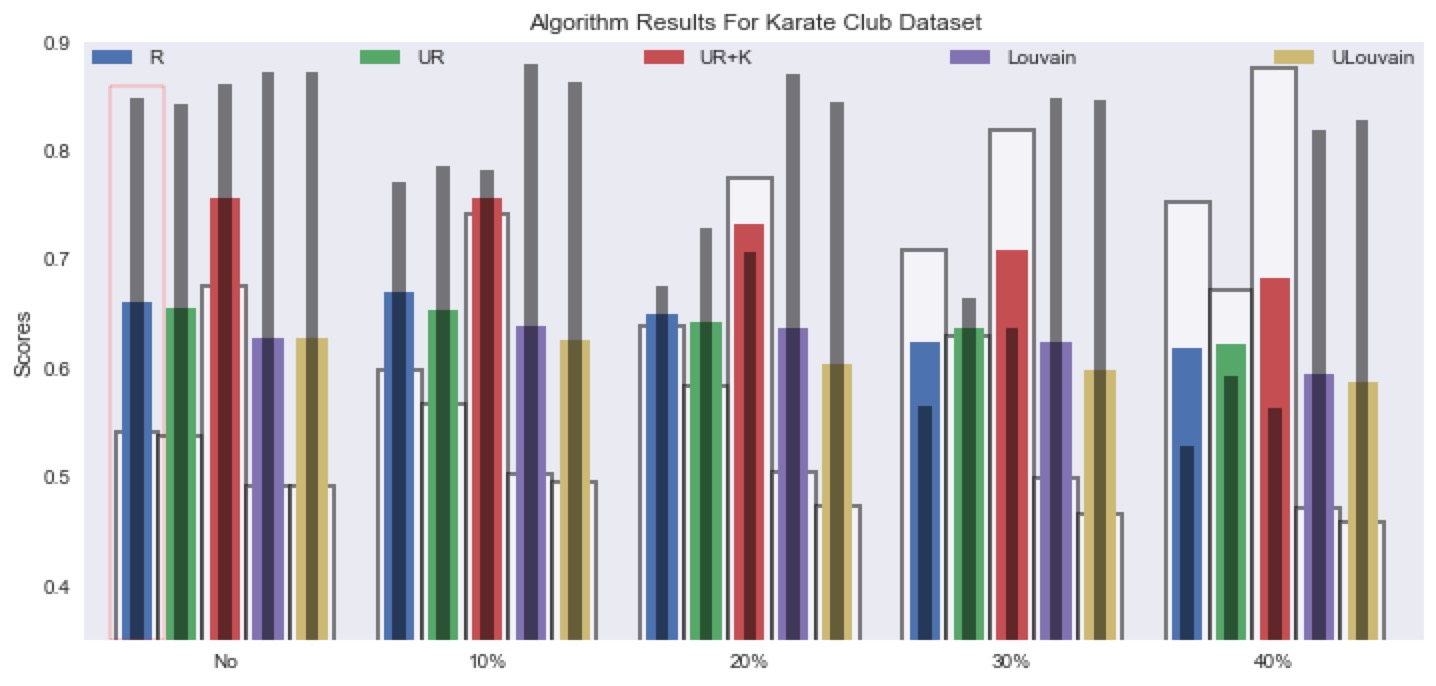
\includegraphics[scale = 0.23]{\main/img/image4.jpeg}
\centering
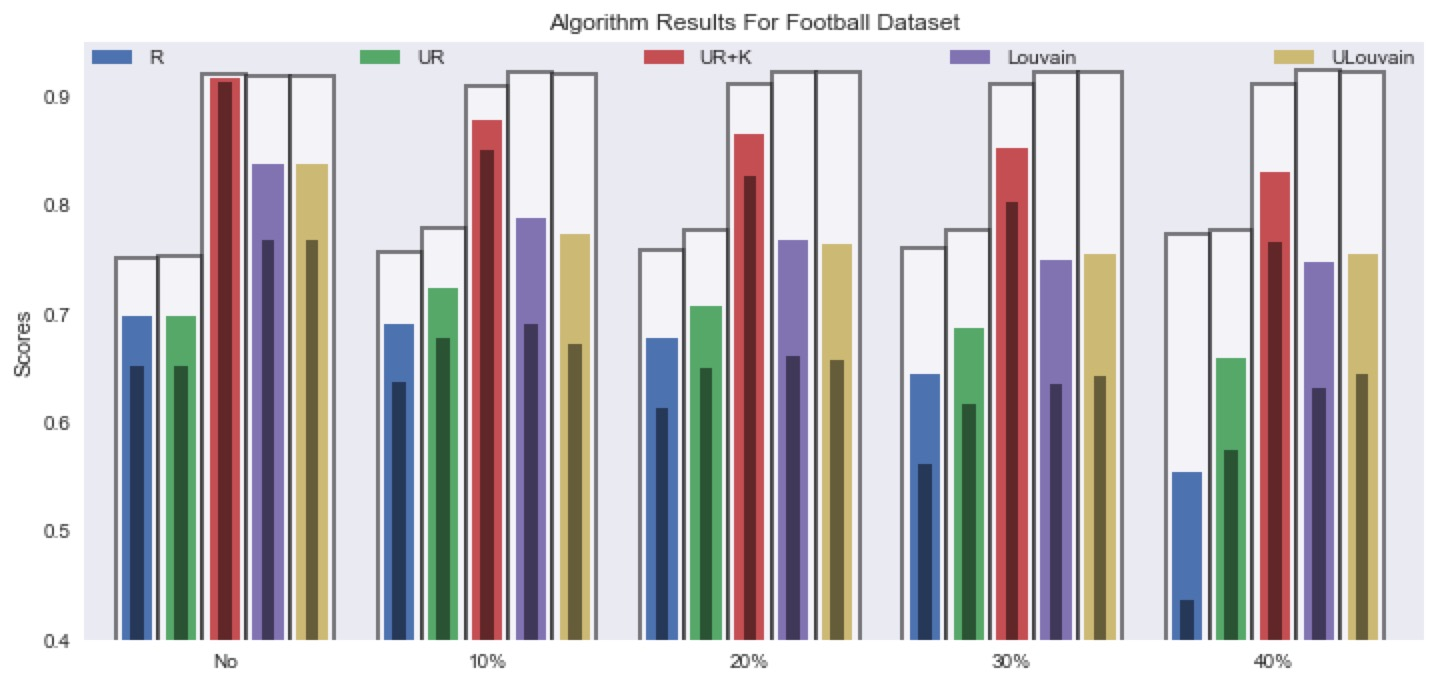
\includegraphics[scale = 0.23]{\main/img/image5.jpeg}
\centering
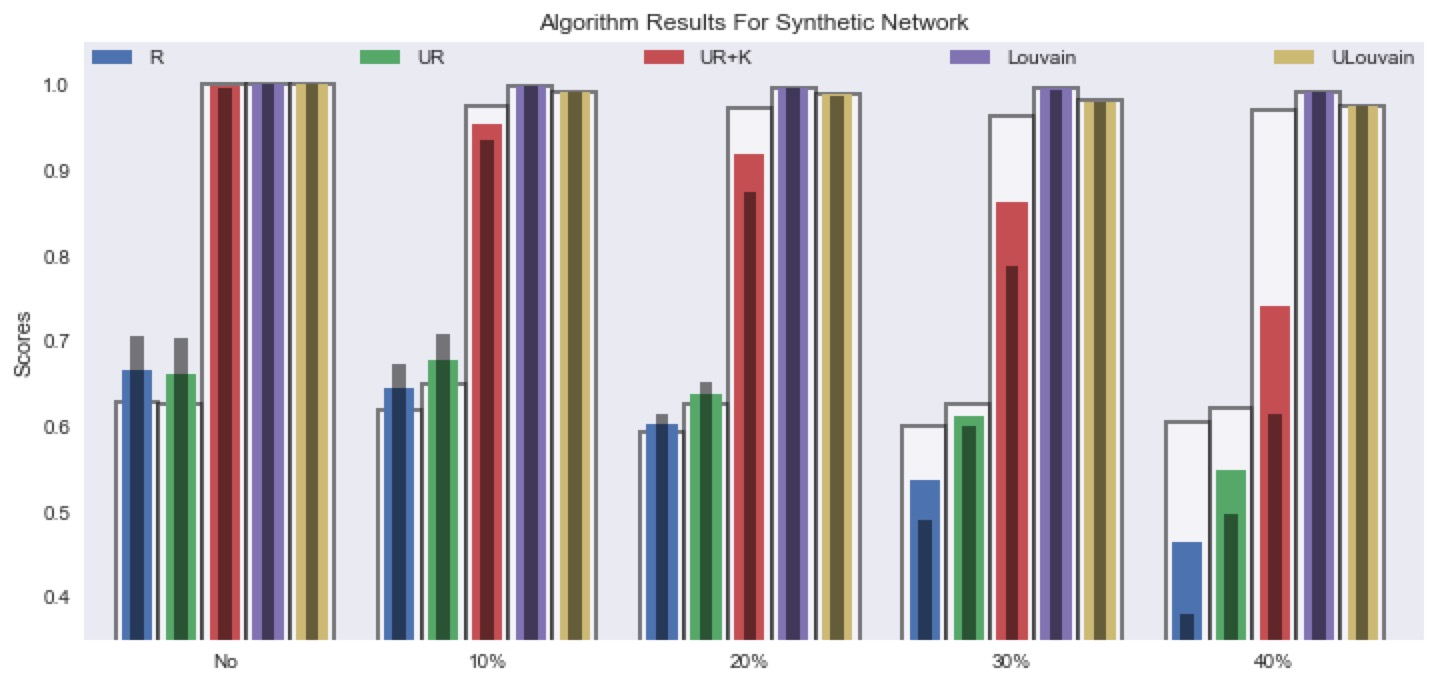
\includegraphics[scale = 0.23]{\main/img/image6.jpeg}
\caption{Algorithm results on karate club, football and synthetic networks. For each network, we add 10\%, 20\%, 30\% and 40\% non-existential edges to the original network. The original network is also regarded as a special case of uncertain network. Therefore, each certain network can generate 5 uncertain networks in total. For each uncertain network, we compare our algorithm (UR+K) with the other 4 algorithms. The precision, recall and f1-measure values of each algorithm are all shown in the graphs. The f1-measure values gained by different algorithms are represented by different colored bars. Each f1-measure value's corresponding precision and recall values are represented by its inner black bar and external white bar respectively. For example, the part wrapped in a red frame represents the results gained by algorithm R on original karate club data. The f1-measure, precision and recall values are 0.6603, 0.848 and 0.5406 respectively.}
\label{supervised-result-local}
\end{figure}

% \begin{figure}[H]
% \includegraphics[scale = 0.23]{image1.jpeg}
% \centering
% \end{figure}
% \begin{figure}[H]
% \includegraphics[scale = 0.23]{image2.jpeg}
% \centering
% \end{figure}
% \begin{figure}[H]
% \includegraphics[scale = 0.23]{image3.jpeg}
% \centering
% \caption{Results}
% \label{cl_enron}
% \end{figure}


% \begin{table}[htbp]
% \begin{center}
% \noindent\makebox[\textwidth]{%
% \begin{tabularx}{1.568\textwidth}{|c|c|c|c|c|c|c|c|c|c|c|c|c|c|c|c|c|c|c|}
% \hline
% \multirow{3}{*}{Noise} & \multicolumn{18}{c|}{Algorithm Results For Karate Club Dataset}                                                                                                                                                                                                              \\ \cline{2-19} 
%                        & \multicolumn{3}{c|}{original R} & \multicolumn{3}{c|}{uncertain R} & \multicolumn{3}{c|}{uncertain R+K} & \multicolumn{3}{c|}{\begin{tabular}[c]{@{}c@{}}uncertain R+K with\\ Examination Phase\end{tabular}} & \multicolumn{3}{c|}{Louvain} & \multicolumn{3}{c|}{ULouvain} \\ \cline{2-19} 
%                        & R         & P        & F1       & R         & P         & F1       & R          & P         & F1        & R                               & P                               & F1                              & R        & P       & F1      & R        & P        & F1      \\ \hline
% No                     & 0.5316  & 0.8347  & 0.6495  & 0.5466  & 0.858  & 0.6678  & 0.7249  & 0.8248  & 0.7716  & 0.7024  & 0.8219  & 0.7575  & 0.4913  & 0.8712  & 0.6283  & 0.4913  & 0.8712  & 0.6283  \\ \hline
% 10\%                   & 0.5612  & 0.7935  & 0.6552  & 0.5349  & 0.816  & 0.6436  & 0.7201  & 0.8278  & 0.7672  & 0.7028  & 0.8397  & 0.7622  & 0.5135  & 0.869  & 0.6427  & 0.4991  & 0.8667  & 0.631  \\ \hline
% 20\%                   & 0.5907  & 0.6828  & 0.6262  & 0.5708  & 0.7194  & 0.6313  & 0.7723  & 0.7537  & 0.7582  & 0.7519  & 0.7796  & 0.7589  & 0.4888  & 0.8516  & 0.6177  & 0.4618  & 0.8118  & 0.5862  \\ \hline
% 30\%                   & 0.7  & 0.6433  & 0.6676  & 0.6104  & 0.7406  & 0.664  & 0.8206  & 0.7328  & 0.7694  & 0.7978  & 0.7476  & 0.7659  & 0.4979  & 0.8753  & 0.6307  & 0.4886  & 0.836  & 0.6131  \\ \hline
% 40\%                   & 0.7721  & 0.5344  & 0.6274  & 0.6115  & 0.6375  & 0.6151  & 0.7865  & 0.67  & 0.7141  & 0.7635  & 0.6809  & 0.708  & 0.4716  & 0.8115  & 0.5929  & 0.4266  & 0.8071  & 0.5553  \\ \hline

% \end{tabularx}}
% \end{center}
% \caption{Algorithm Results For Karate Club Dataset}
% \end{table}

% \begin{table}[htbp]
% \begin{center}
% \noindent\makebox[\textwidth]{%
% \begin{tabularx}{1.568\textwidth}{|c|c|c|c|c|c|c|c|c|c|c|c|c|c|c|c|c|c|c|}
% \hline
% \multirow{3}{*}{Noise} & \multicolumn{18}{c|}{Algorithm Results For Football Dataset}                                                                                                                                                                                                              \\ \cline{2-19} 
%                        & \multicolumn{3}{c|}{original R} & \multicolumn{3}{c|}{uncertain R} & \multicolumn{3}{c|}{uncertain R+K} & \multicolumn{3}{c|}{\begin{tabular}[c]{@{}c@{}}uncertain R+K with\\ Examination Phase\end{tabular}} & \multicolumn{3}{c|}{Louvain} & \multicolumn{3}{c|}{ULouvain} \\ \cline{2-19} 
%                        & R         & P        & F1       & R         & P         & F1       & R          & P         & F1        & R                               & P                               & F1                              & R        & P       & F1      & R        & P        & F1      \\ \hline
% No                     & 0.7512  & 0.6548  & 0.6997  & 0.7573  & 0.6599  & 0.7052  & 0.9208  & 0.9106  & 0.9156  & 0.9147  & 0.9227  & 0.9187  & 0.919  & 0.7682  & 0.8369  & 0.919  & 0.7682  & 0.8369  \\ \hline
% 10\%                   & 0.7727  & 0.6488  & 0.7051  & 0.787  & 0.6877  & 0.7334  & 0.9075  & 0.8475  & 0.876  & 0.877  & 0.8856  & 0.881  & 0.9211  & 0.6825  & 0.7817  & 0.9214  & 0.6603  & 0.766  \\ \hline
% 20\%                   & 0.7721  & 0.6401  & 0.6993  & 0.7885  & 0.6716  & 0.7248  & 0.9111  & 0.8426  & 0.8752  & 0.8599  & 0.8872  & 0.8731  & 0.9245  & 0.6703  & 0.7755  & 0.9217  & 0.7076  & 0.7983  \\ \hline
% 30\%                   & 0.7638  & 0.5681  & 0.6508  & 0.7748  & 0.6054  & 0.6787  & 0.9137  & 0.7852  & 0.8434  & 0.8047  & 0.8286  & 0.8151  & 0.9223  & 0.6237  & 0.7422  & 0.9229  & 0.6805  & 0.7792  \\ \hline
% 40\%                   & 0.7592  & 0.4413  & 0.5569  & 0.7736  & 0.5432  & 0.6355  & 0.9085  & 0.7346  & 0.8093  & 0.766  & 0.7696  & 0.7638  & 0.9236  & 0.6168  & 0.7371  & 0.9204  & 0.6841  & 0.7815  \\ \hline

% \end{tabularx}}
% \end{center}
% \caption{Algorithm Results For Football Dataset}
% \end{table}

% \begin{table}[htbp]
% \begin{center}
% \noindent\makebox[\textwidth]{%
% \begin{tabularx}{1.568\textwidth}{|c|c|c|c|c|c|c|c|c|c|c|c|c|c|c|c|c|c|c|}
% \hline
% \multirow{3}{*}{Noise} & \multicolumn{18}{c|}{Algorithm Results For Synthetic Network}                                                                                                                                                                                                              \\ \cline{2-19} 
%                        & \multicolumn{3}{c|}{original R} & \multicolumn{3}{c|}{uncertain R} & \multicolumn{3}{c|}{uncertain R+K} & \multicolumn{3}{c|}{\begin{tabular}[c]{@{}c@{}}uncertain R+K with\\ Examination Phase\end{tabular}} & \multicolumn{3}{c|}{Louvain} & \multicolumn{3}{c|}{ULouvain} \\ \cline{2-19} 
%                        & R         & P        & F1       & R         & P         & F1       & R          & P         & F1        & R                               & P                               & F1                              & R        & P       & F1      & R        & P        & F1      \\ \hline
% No                     & 0.6301  & 0.7057  & 0.6657  & 0.6254  & 0.7033  & 0.6621  & 1.0  & 1.0  & 1.0  & 1.0  & 1.0  & 1.0  & 1.0  & 1.0  & 1.0  & 1.0  & 1.0  & 1.0  \\ \hline
% 10\%                  & 0.6217  & 0.6686  & 0.6442  & 0.6474  & 0.6922  & 0.6688  & 0.974  & 0.9288  & 0.9501  & 0.9545  & 0.9579  & 0.9557  & 0.9969  & 0.9971  & 0.997  & 0.9817  & 0.9802  & 0.9809  \\ \hline
% 20\%                   & 0.6012  & 0.6023  & 0.6014  & 0.6526  & 0.6679  & 0.6597  & 0.9711  & 0.8762  & 0.9194  & 0.9325  & 0.9151  & 0.9217  & 0.9911  & 0.9922  & 0.9917  & 0.9823  & 0.9802  & 0.9812  \\ \hline
% 30\%                   & 0.628  & 0.5332  & 0.5728  & 0.6348  & 0.619  & 0.6257  & 0.969  & 0.855  & 0.9053  & 0.9044  & 0.8996  & 0.8982  & 0.9852  & 0.9865  & 0.9859  & 0.9706  & 0.9681  & 0.9694  \\ \hline
% 40\%                   & 0.7049  & 0.3795  & 0.4872  & 0.643  & 0.4804  & 0.547  & 0.967  & 0.6737  & 0.7854  & 0.8871  & 0.7072  & 0.7751  & 0.9773  & 0.9711  & 0.9736  & 0.952  & 0.9541  & 0.953  \\ \hline

% \end{tabularx}}
% \end{center}
% \caption{Algorithm Results For Synthetic Network}
% \end{table}

From Figure \ref{supervised-result-local}, we can observe that our algorithm (UR+K) can significantly outperform other algorithms in terms of f1-measure in karate club dataset and football dataset. Though our algorithm can not beat Louvain and ULouvain algorithms in synthetic network, it also shows competitive detection accuracy, and it still performs better than algorithms R and UR on synthetic dataset. Considering our algorithm only use local information, while Louvain and ULouvain use global information, these results are still satisfying. %(NEED POLISHED)

% When we compare results achieved by our algorithm (uncertain R+K with Examination Phase) and uncertain R+K, we find that they gain almost the same f1-measure value. The former one has higher recall value, while its precision value is lower. We can also find that our algorithm tends to perform better when networks have more noises, while it is slightly worse than uncertain R+K when networks are more certain. (NEED POLISHED)

% However, there exists a problem. we have an assumption, we assume that the community structure does not change when we add noises.

% \begin{table}[]
% \centering
% \caption{My caption}
% \label{my-label}
% \begin{tabular}{|c|c|c|c|c|c|c|c|c|c|c|c|c|c|c|c|c|c|c|c|c|c|c|c|c|}
% \hline
% \multirow{3}{*}{Noise} & \multicolumn{24}{c|}{Algorithm Results For Karate Club Dataset}                                                                                                                                                                                                                                                                                          \\ \cline{2-25} 
%                        & \multicolumn{3}{c|}{original R} & \multicolumn{3}{c|}{uncertain R} & \multicolumn{3}{c|}{uncertain R+K} & \multicolumn{3}{c|}{\begin{tabular}[c]{@{}c@{}}uncertain R+K with\\ Examination Phase\end{tabular}} & \multicolumn{3}{c|}{Louvain} & \multicolumn{3}{c|}{ULouvain} & \multicolumn{3}{c|}{uncertain R+K/} & \multicolumn{3}{c|}{uncertain R+K-} \\ \cline{2-25} 
%                        & P         & R        & F1       & P         & R         & F1       & P          & R         & F1        & P                               & R                               & F1                              & P        & R       & F1      & P        & R        & F1      & P          & R          & F1        & P          & R          & F1        \\ \hline
% No                     & 0.5395    & 0.8465   & 0.659    & 0.5396    & 0.8453    & 0.6587   & 0.7232     & 0.8023    & 0.7607    & 0.7145                          & 0.8082                          & 0.7585                          & 0.4913   & 0.8712  & 0.6283  & 0.4913   & 0.8712   & 0.6283  & 0.5779     & 0.8329     & 0.6823    & 0.6298     & 0.833      & 0.7172    \\ \hline
% 10\%                   & 0.5566    & 0.7868   & 0.6486   & 0.5573    & 0.8089    & 0.657    & 0.7412     & 0.7561    & 0.7463    & 0.7231                          & 0.7681                          & 0.7425                          & 0.5028   & 0.8734  & 0.6366  & 0.4937   & 0.8634   & 0.6259  & 0.6489     & 0.7291     & 0.6806    & 0.6391     & 0.7457     & 0.6829    \\ \hline
% 20\%                   & 0.6287    & 0.7068   & 0.659    & 0.5689    & 0.7523    & 0.643    & 0.7595     & 0.7284    & 0.7405    & 0.7395                          & 0.7375                          & 0.7351                          & 0.4894   & 0.8522  & 0.6193  & 0.4731   & 0.8413   & 0.6031  & 0.6909     & 0.662      & 0.6694    & 0.6758     & 0.6763     & 0.6691    \\ \hline
% 35\%                   & 0.7311    & 0.5834   & 0.641    & 0.6077    & 0.6622    & 0.6254   & 0.7885     & 0.6592    & 0.7142    & 0.7698                          & 0.6638                          & 0.7085                          & 0.4742   & 0.8247  & 0.5995  & 0.4447   & 0.8174   & 0.5738  & 0.7407     & 0.5676     & 0.6367    & 0.7292     & 0.582      & 0.6407    \\ \hline
% 50\%                   & 0.8151    & 0.5309   & 0.6388   & 0.6571    & 0.604     & 0.6212   & 0.8292     & 0.6191    & 0.7062    & 0.8137                          & 0.6237                          & 0.703                           & 0.4516   & 0.7855  & 0.5702  & 0.4257   & 0.7925   & 0.5507  & 0.7857     & 0.5419     & 0.6371    & 0.7763     & 0.5503     & 0.639     \\ \hline
% \end{tabular}
% \end{table}

\subsection*{Unsupervised Evaluation}
Since we generate uncertain networks based on certain networks. When we evaluate our algorithm in the supervised way, we assume that uncertain networks have the same community ground truth as their corresponding certain networks. This assumption is true if we only add a few noise edges to uncertain networks because small number of noise edges will not have impact on the community structure. However, with the increase in the number of noise edges, some communities may merge into one community. In this scenario, using original community labels will cause problems.

To solve this problem, we also propose an unsupervised way to evaluate our algorithm. As mentioned in Section \ref{Local-Community-Detection-Algorithms-Review}, the local community modularity $\mathcal{R}$ can be used to measure the quality of the local community. In the uncertain networks scenario, we can use $\mathcal{UR}$ to take the place of $\mathcal{R}$. Therefore, to compare different algorithms, we can compare local community modularity $\mathcal{UR}$ values after running different algorithms.

In this part, we also compare our algorithm (UR+K) with other algorithms on 2 real-networks and 1 synthetic network. The results are shown in Table \ref{unsupervised_karate}, \ref{unsupervised_football}, \ref{unsupervised_synthetic}.

% Another way to evaluate our algorithm is the unsupervised way. We can compare modularity values after running different algorithms. In this part, we use two different local modularities: (1) the first is $\mathcal{UR}$, which have already been defined in equation(2) and have been used to merge new nodes to existing community; and (2) a new modularity, $sample\mathcal{R}$, to evaluate different algorithms. $sample\mathcal{R}$ is a sample-based modularity, which  can be represented as:
% \begin{equation}
% sample\mathcal{R} = \frac{1}{N}\sum_{i=1}^{N}\mathcal{R}_i
% \end{equation}
% Given uncertain network $\mathcal{G = (V,E,P)}$, we can sample each edge in $\mathcal{G}$ according to the probability $p(e)$ to generate the possible graph $G = (V_G,E_G)$. We have $E_G \in \mathcal{E}$ and $V_G \in \mathcal{E}$. The probability $Pr|G|$ of sampling the possible graph is as follows:
% \begin{equation}
% Pr|G| = \prod_{e\in E_G}p(e)\prod_{e\in \mathcal{E}, e\notin E_G}(1-p(e))
% \end{equation}
% There are a total of $2^{|\mathcal{E}|}$ possible graphs, since each edge provides us with a binary sampling decision. The number of possible graphs become very large with the increase of number of edges. After running each algorithm, we have the local community for each start node. In evaluation, we can sample enough (e.g. 1000) possible graphs and calculate the modularity $\mathcal{R}$ based on equation (1) for each possible graph. Then we can get the $sample\mathcal{R}$ for each algorithm according to equation (13).
%According to Chernoff-Hoeffding Bound

\begin{table}[]
\centering
\caption{$\mathcal{UR}$ on Karate Club Data}
\label{unsupervised_karate}
\begin{tabular}{|c|c|c|c|c|c|}
\hline
Noise & R      & UR     & UR+K            & Louvain & ULouvain \\ \hline
No    & 0.5787 & 0.5789 & \textbf{0.654}  & 0.5604  & 0.5604   \\ \hline
10\%  & 0.584  & 0.5902 & \textbf{0.7026} & 0.5176  & 0.5258   \\ \hline
20\%  & 0.6235 & 0.5942 & \textbf{0.7462} & 0.4737  & 0.4858   \\ \hline
30\%  & 0.7065 & 0.6232 & \textbf{0.7858} & 0.4326  & 0.4583   \\ \hline
40\%  & 0.7628 & 0.6641 & \textbf{0.8601} & 0.3965  & 0.4281   \\ \hline
\end{tabular}
\end{table}

% \begin{table}[]
% \centering
% \caption{$\mathcal{UR}$ on Karate Club Data}
% \label{my-label}
% \begin{tabular}{|c|c|c|c|c|c|c|}
% \hline
% Noise & original R & uncertain R & uncertain R+K & \begin{tabular}[c]{@{}c@{}}uncertain R+K with \\ Examination Phase\end{tabular} & Louvain & ULouvain \\ \hline
% No    &  0.5783&  0.5788&  0.654&  0.6507&  0.5604&  0.5604  \\ \hline
% 10\%  &  0.5641&  0.5904&  0.6726&  0.6566&  0.5364&  0.5467  \\ \hline
% 20\%  &  0.5869&  0.5759&  0.6894&  0.6708&  0.4799&  0.5125  \\ \hline
% 30\%  &  0.7243&  0.6193&  0.7487&  0.7358&  0.4631&  0.4589  \\ \hline
% 40\%  &  0.7615&  0.6205&  0.7644&  0.7492&  0.4015&  0.4508  \\ \hline
% \end{tabular}
% \end{table}

% \begin{table}[]
% \centering
% \caption{$Sample\mathcal{R}$ on Karate Club Data}
% \label{my-label}
% \begin{tabular}{|c|c|c|c|c|c|c|}
% \hline
% Noise & original R & uncertain R & uncertain R+K & \begin{tabular}[c]{@{}c@{}}uncertain R+K with \\ Examination Phase\end{tabular} & Louvain & ULouvain \\ \hline
% No    &  0.5783&  0.5788&  0.654&  0.6507&  0.5604&  0.5604  \\ \hline
% 10\%  &  0.522&  0.5454&  0.6158&  0.6089&  0.5068&  0.5213  \\ \hline
% 20\%  &  0.5505&  0.5372&  0.6361&  0.6244&  0.4583&  0.4909  \\ \hline
% 30\%  &  0.701&  0.5822&  0.7019&  0.696&  0.4442&  0.4388  \\ \hline
% 40\%  &  0.741&  0.587&  0.7231&  0.711&  0.3878&  0.4376  \\ \hline
% \end{tabular}
% \end{table}

\begin{table}[]
\centering
\caption{$\mathcal{UR}$ on Football Data}
\label{unsupervised_football}
\begin{tabular}{|c|c|c|c|c|c|}
\hline
Noise & R      & UR     & UR+K   & Louvain         & ULouvain        \\ \hline
No    & 0.5065 & 0.5057 & 0.5327 & \textbf{0.5497} & \textbf{0.5497} \\ \hline
10\%  & 0.4714 & 0.4826 & 0.4902 & 0.5152          & \textbf{0.5208} \\ \hline
20\%  & 0.4378 & 0.4491 & 0.454  & 0.4783          & \textbf{0.4802} \\ \hline
30\%  & 0.415  & 0.4189 & 0.4221 & 0.4384          & \textbf{0.4463} \\ \hline
40\%  & 0.4121 & 0.4008 & 0.4017 & 0.4134          & \textbf{0.4164} \\ \hline
\end{tabular}
\end{table}

% \begin{table}[]
% \centering
% \caption{$\mathcal{UR}$ on Football Data}
% \label{my-label}
% \begin{tabular}{|c|c|c|c|c|c|c|}
% \hline
% Noise & original R & uncertain R & uncertain R+K & \begin{tabular}[c]{@{}c@{}}uncertain R+K with \\ Examination Phase\end{tabular} & Louvain & ULouvain \\ \hline
% No    &  0.5066&  0.5054&  0.5327&  0.5254&  0.5497&  0.5497  \\ \hline
% 10\%  &  0.4693&  0.4868&  0.4938&  0.4762&  0.518&  0.5217  \\ \hline
% 20\%  &  0.4363&  0.4495&  0.455&  0.4219&  0.4804&  0.4792  \\ \hline
% 30\%  &  0.4172&  0.4189&  0.4203&  0.37&  0.4391&  0.4358  \\ \hline
% 40\%  &  0.4138&  0.4011&  0.3994&  0.3343&  0.4145&  0.4243  \\ \hline
% \end{tabular}
% \end{table}

% \begin{table}[]
% \centering
% \caption{$Sample\mathcal{R}$ on Football Data}
% \label{my-label}
% \begin{tabular}{|c|c|c|c|c|c|c|}
% \hline
% Noise & original R & uncertain R & uncertain R+K & \begin{tabular}[c]{@{}c@{}}uncertain R+K with \\ Examination Phase\end{tabular} & Louvain & ULouvain \\ \hline
% No    &  0.5066&  0.5054&  0.5327&  0.5254&  0.5497&  0.5497  \\ \hline
% 10\%  &  0.4682&  0.4855&  0.493&  0.4757&  0.5156&  0.5192  \\ \hline
% 20\%  &  0.4359&  0.449&  0.4548&  0.4219&  0.4791&  0.4786  \\ \hline
% 30\%  &  0.4163&  0.4186&  0.4201&  0.3699&  0.4384&  0.4354  \\ \hline
% 40\%  &  0.4123&  0.401&  0.3994&  0.3343&  0.4147&  0.4242  \\ \hline
% \end{tabular}
% \end{table}

\begin{table}[]
\centering
\caption{$\mathcal{UR}$ on Synthetic Data}
\label{unsupervised_synthetic}
\begin{tabular}{|c|c|c|c|c|c|}
\hline
Noise & R      & UR     & UR+K            & Louvain         & ULouvain        \\ \hline
No    & 0.6018 & 0.6019 & \textbf{0.6537} & \textbf{0.6537} & \textbf{0.6537} \\ \hline
10\%  & 0.5476 & 0.5361 & \textbf{0.5928} & 0.5924          & 0.5924          \\ \hline
20\%  & 0.5016 & 0.4941 & \textbf{0.5484} & 0.5415          & 0.5414          \\ \hline
30\%  & 0.4964 & 0.4685 & \textbf{0.5306} & 0.5003          & 0.5             \\ \hline
40\%  & 0.5232 & 0.4735 & \textbf{0.5742} & 0.4635          & 0.4642          \\ \hline
\end{tabular}
\end{table}

% \begin{table}[]
% \centering
% \caption{$\mathcal{UR}$ on Synthetic Data}
% \label{my-label}
% \begin{tabular}{|c|c|c|c|c|c|c|}
% \hline
% Noise & original R & uncertain R & uncertain R+K & \begin{tabular}[c]{@{}c@{}}uncertain R+K with \\ Examination Phase\end{tabular} & Louvain & ULouvain \\ \hline
% No    &  0.6017&  0.602&  0.6537&  0.6537&  0.6537&  0.6537  \\ \hline
% 10\%  &  0.5553&  0.5571&  0.6014&  0.596&  0.5995&  0.6  \\ \hline
% 20\%  &  0.5041&  0.4957&  0.5484&  0.5346&  0.5399&  0.5418  \\ \hline
% 30\%  &  0.4759&  0.4729&  0.5285&  0.5081&  0.5038&  0.505  \\ \hline
% 40\%  &  0.56&  0.4618&  0.5008&  0.4721&  0.4683&  0.4712  \\ \hline
% \end{tabular}
% \end{table}

% \begin{table}[]
% \centering
% \caption{$Sample\mathcal{R}$ on Synthetic Data}
% \label{my-label}
% \begin{tabular}{|c|c|c|c|c|c|c|}
% \hline
% Noise & original R & uncertain R & uncertain R+K & \begin{tabular}[c]{@{}c@{}}uncertain R+K with \\ Examination Phase\end{tabular} & Louvain & ULouvain \\ \hline
% No    &  0.6017&  0.602&  0.6537&  0.6537&  0.6537&  0.6537  \\ \hline
% 10\%  &  0.5499&  0.5519&  0.5977&  0.5927&  0.596&  0.5965  \\ \hline
% 20\%  &  0.5015&  0.4934&  0.5471&  0.5337&  0.5388&  0.5407  \\ \hline
% 30\%  &  0.4741&  0.4709&  0.5267&  0.5067&  0.5035&  0.5046  \\ \hline
% 40\%  &  0.5588&  0.4607&  0.5002&  0.4717&  0.4683&  0.4713  \\ \hline
% \end{tabular}
% \end{table}

From Table \ref{unsupervised_karate}, \ref{unsupervised_football}, \ref{unsupervised_synthetic}, we can find our algorithm (UR+K) performs the best on karate club and synthetic datasets, and the $\mathcal{UR}$ values achieved on football dataset by our algorithm are very close to the best results achieved by the  other algorithms. It is worth noting that, in the expansion steps, though UR algorithm always choose the node which gives the largest increase of $\mathcal{UR}$, while $\mathcal{UR}$ value is not mainly considered in the first few steps in our algorithm, our algorithm finally achieved higher $\mathcal{UR}$ values than UR algorithm on all datasets.

\subsection{Hyper-Parameter Evaluation} \label{Hyper-Parameter-Evaluation-Local}
Our algorithm has a hyper-parameter $\lambda$. As we mentioned in Section \ref{Full-Algorithm-Description-local}, the choice of hyper-parameter $\lambda$ is another crucial topic in our experiment. To validate that the $\lambda$ value we use is a reasonable choice, we conduct experiments in this section to find optimal $\lambda$. We do this by repeating previous supervised evaluation experiments on karate club, football and synthetic networks over a range of different $\lambda$ values, as shown in Figure \ref{Hyper-Parameter-Evaluation-local-graph}. 

By using different $\lambda$ values, we run our algorithm (UR+K) on three networks and get their corresponding f1-measure values. 

\begin{figure}
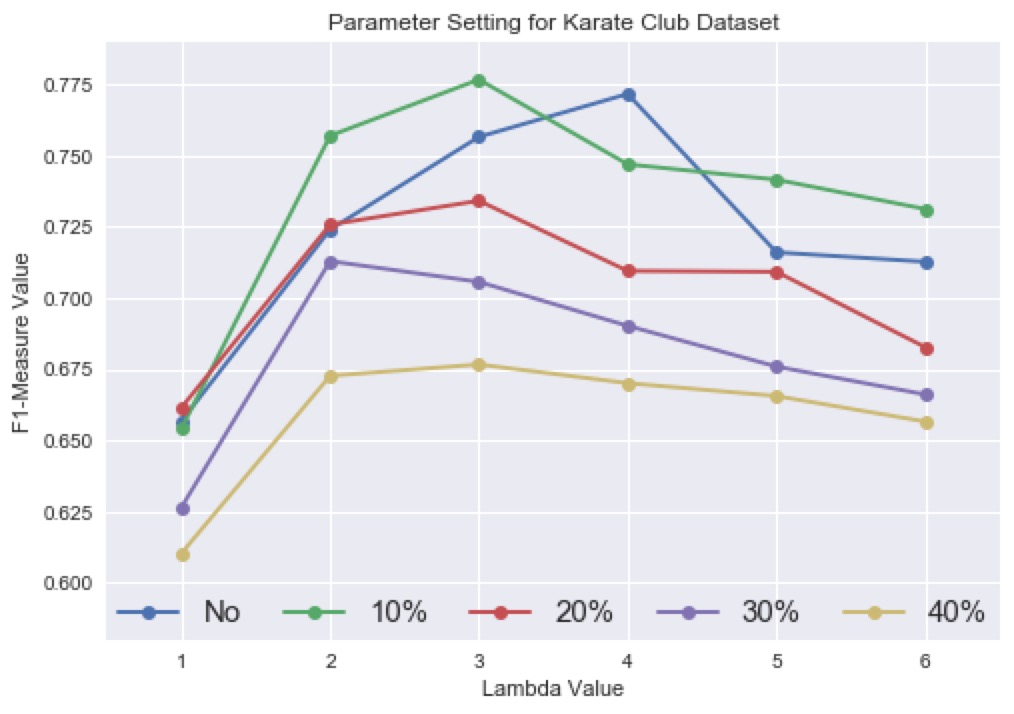
\includegraphics[scale = 0.17]{\main/img/para1.jpeg}
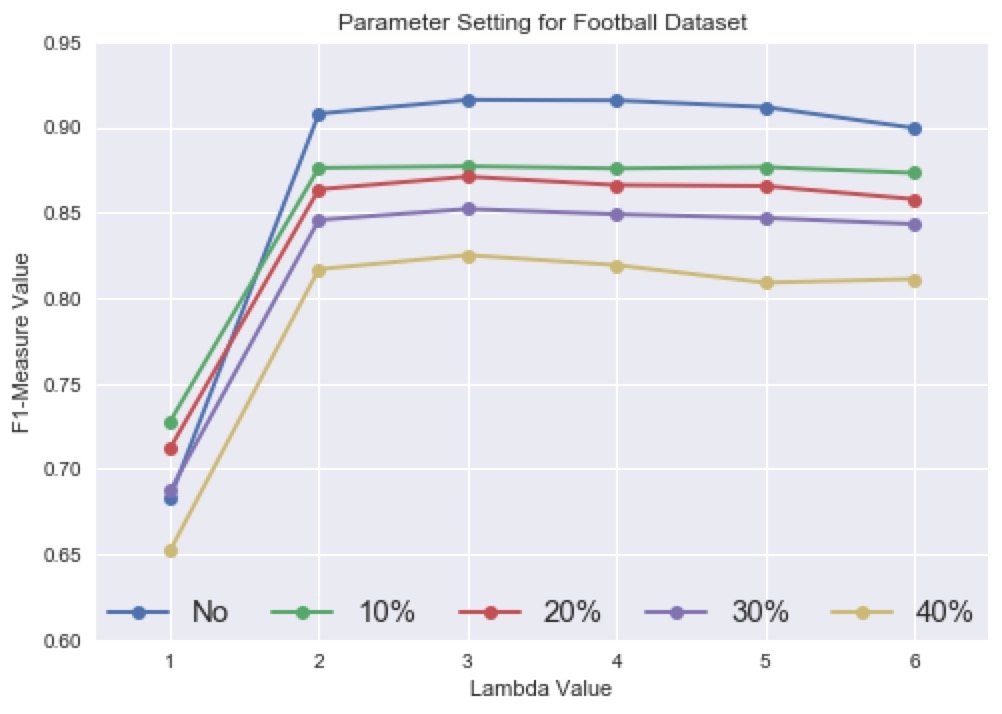
\includegraphics[scale = 0.17]{\main/img/para2.jpeg}
\centering
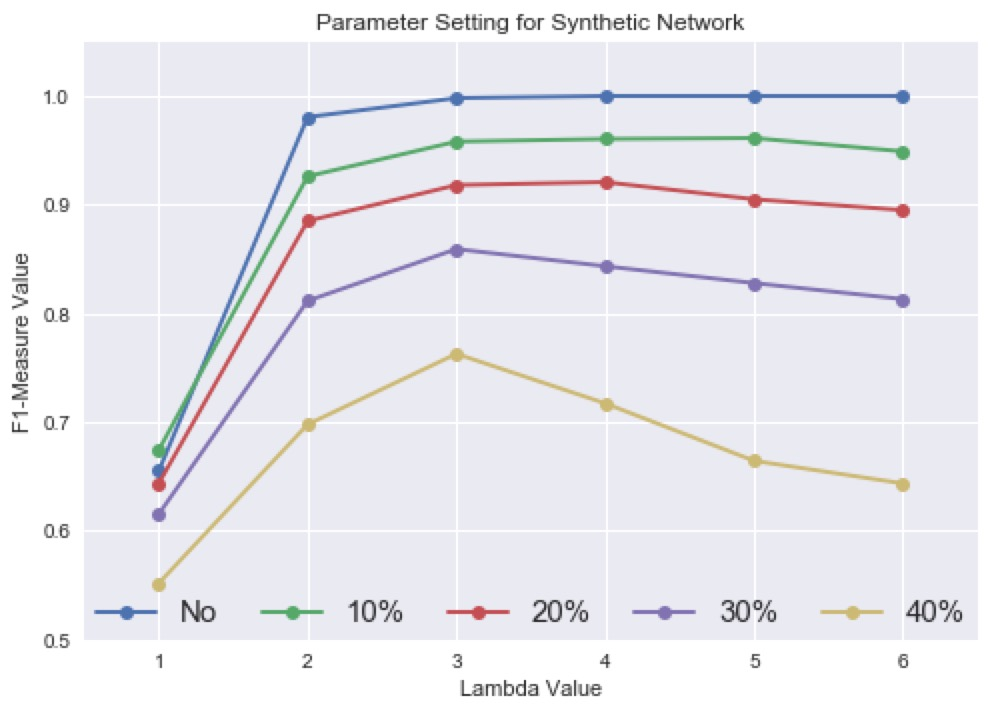
\includegraphics[scale = 0.17]{\main/img/para3.jpeg}
\caption{Hyper-parameter Validation}
\label{Hyper-Parameter-Evaluation-local-graph}
\end{figure}

From these experiments, we can conclude that though the optimal choice of the hyper-parameter $\lambda$ varies with networks, the best choice of the hyper-parameter $\lambda$ is 3 or 4 in almost all cases. In most cases, $\lambda=3$ performs the best compared to the other values. Even in the other cases when $\lambda=3$ is not the optimal choice, the results achieved by $\lambda=3$ is also competitive compared to the results achieved by the optimal $\lambda$ value. Therefore, it is reasonable to choose $\lambda=3$ when run our algorithm.

\section{Conclusion}
In this Chapter, we provide a novel approach which is able to detect local communities in uncertain networks. By taking the new measure $\mathcal{K}$ into consideration, our algorithm can outperform the other local community detection algorithm based on supervised and unsupervised evaluations.

\end{document}